\documentclass[11pt]{article}
\usepackage{float}
\usepackage{amsmath}
\usepackage{graphicx}
\usepackage{geometry}
\usepackage[hidelinks]{hyperref}
\usepackage{titlesec}
\usepackage{subcaption}
\usepackage{listings}
\usepackage{xcolor}

\lstset{
  basicstyle=\ttfamily\footnotesize,
  keywordstyle=\color{blue},
  commentstyle=\color{gray},
  numbers=left,
  numberstyle=\tiny,
  breaklines=true,
  frame=single,
  tabsize=4
}

\geometry{margin=1in}
\titleformat{\section}{\normalfont\Large\bfseries}{\thesection}{1em}{}
\titleformat{\subsection}{\normalfont\large\bfseries}{\thesubsection}{1em}{}

\title{Optimization Techniques: Exercise 1}
\author{Maria Charisi 10727}
\date{November 2025\\ 
\href{https://github.com/mariaxarisi/Optimization-Techniques}{\texttt{Github Repo}}}

\begin{document}

\maketitle

\begin{abstract}
This report constitutes the first part of the assignment for the \textit{Optimization Techniques} course at the \textit{Aristotle University of Thessaloniki}. Its objective is to implement four different optimization methods in MATLAB to determine the minima of given convex functions. The report presents a brief theoretical description of each method, followed by the corresponding implementation details, graphical results, and a discussion of the observed performance of the algorithms.
\end{abstract}

\tableofcontents
\newpage

\section{Introduction}

In this report, we study and compare four optimization methods applied to convex functions. Specifically, we consider three functions that are convex in the interval $[-1, 3]$:

\begin{align}
    f_1(x) &= 5^{x} + (2 - \cos{x})^2, \\
    f_2(x) &= (x - 1)^2 + e^{(x - 5)} \sin{(x + 3)}, \\
    f_3(x) &= e^{-3x} - (\sin{(x - 2)} - 2)^2.
\end{align}

We will apply and compare the following optimization techniques to estimate the minima of the given functions:
\begin{itemize}
    \item Dichotomy Method
    \item Golden Section Method
    \item Fibonacci Method
    \item Dichotomy Method with Derivatives
\end{itemize}

A visual representation of the three functions within the interval $[-1, 3]$ is shown in Figure~\ref{fig:functions}.

\begin{figure}[h!]
    \centering
    \begin{subfigure}[b]{0.32\textwidth}
        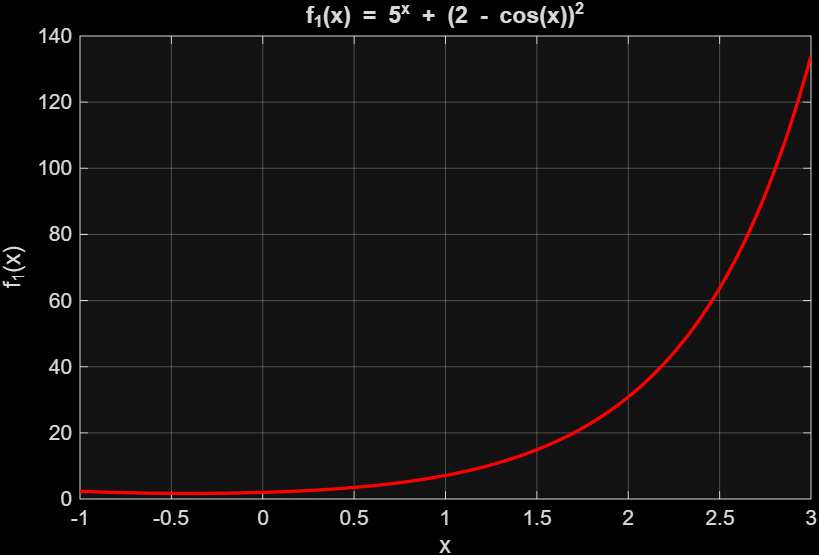
\includegraphics[width=\textwidth]{assets/f1.png}
        \caption{$f_1(x)$}
    \end{subfigure}
    \hfill
    \begin{subfigure}[b]{0.32\textwidth}
        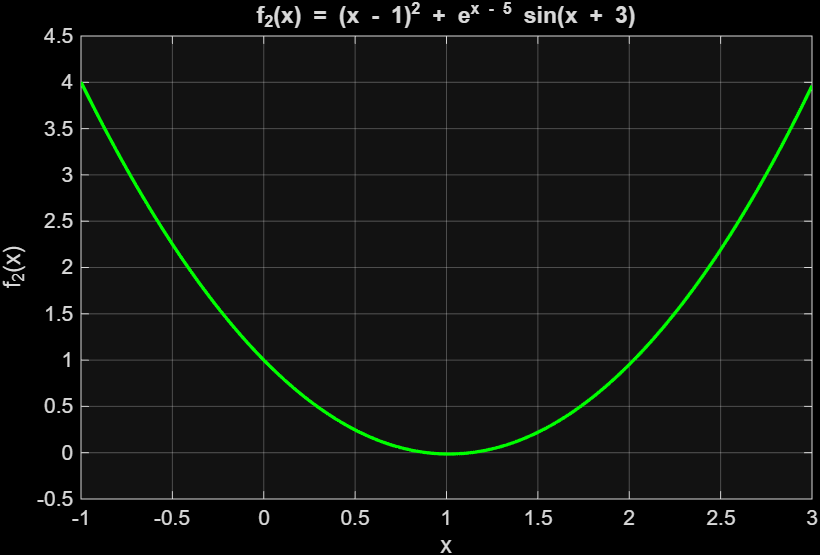
\includegraphics[width=\textwidth]{assets/f2.png}
        \caption{$f_2(x)$}
    \end{subfigure}
    \hfill
    \begin{subfigure}[b]{0.32\textwidth}
        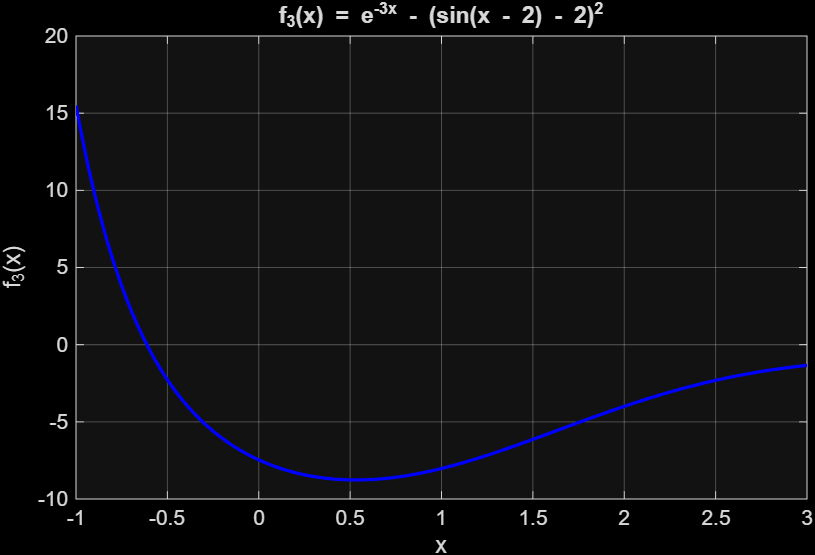
\includegraphics[width=\textwidth]{assets/f3.png}
        \caption{$f_3(x)$}
    \end{subfigure}
    \caption{Plots of the three convex functions in the interval $[-1, 3]$.}
    \label{fig:functions}
\end{figure}

\section{Dichotomy Method}

\subsection{Method Description}

The Dichotomy Method is a technique for locating the minimum of a function within a given interval $[a, b]$. The method iteratively reduces the search interval by evaluating the function at two points placed symmetrically around the midpoint.

At each iteration, two evaluation points are defined as:
\[
x_1 = \frac{a + b}{2} - \varepsilon, \quad
x_2 = \frac{a + b}{2} + \varepsilon,
\]
where $\varepsilon$ is a small positive constant ensuring that $x_1$ and $x_2$ are distinct.  
The function values $f(x_1)$ and $f(x_2)$ are compared:

\[
\text{If } f(x_1) < f(x_2), \text{ then } b = x_2; \quad
\text{otherwise, } a = x_1.
\]

This process repeats until the length of the current interval satisfies:
\[
(b - a) < l,
\]
where $l$ is the desired precision.  
The midpoint of the final interval is taken as the estimated minimizer:
\[
x_{\text{min}} = \frac{a + b}{2}.
\]

The following code, shown in Listing \ref{lst:dichotomy}, presents the MATLAB implementation of the Dichotomy Method.

\begin{lstlisting}[language=Matlab, caption={Implementation of the Dichotomy Method in MATLAB}, label={lst:dichotomy}]
function [min_x, min_f, num_calculations, k, ak_vector, bk_vector] = dichotomy_method(f, a, b, l, e)
    num_calculations = 0;
    k = 1;
    ak_vector = a;
    bk_vector = b;

    while (b - a) > l
        c = (a + b) / 2;
        x1 = c - e;
        x2 = c + e;

        fx1 = f(x1);
        fx2 = f(x2);
        num_calculations = num_calculations + 2;

        if fx1 < fx2
            b = x2; % minimum in left half
        elseif fx1 > fx2
            a = x1; % minimum in right half
        else
            a = x1;
            b = x2;
        end

        ak_vector = [ak_vector, a];
        bk_vector = [bk_vector, b];
        k = k + 1;
    end

    min_x = (a + b) / 2;
    min_f = f(min_x);
end
\end{lstlisting}

\subsection{Plots and Observations}

In this subsection, we present the numerical results of applying the Dichotomy Method to the three test functions.  
The behavior of the method is analyzed by examining the number of function evaluations under different parameters, as well as the convergence of the interval endpoints.

\begin{figure}[h!]
    \centering
    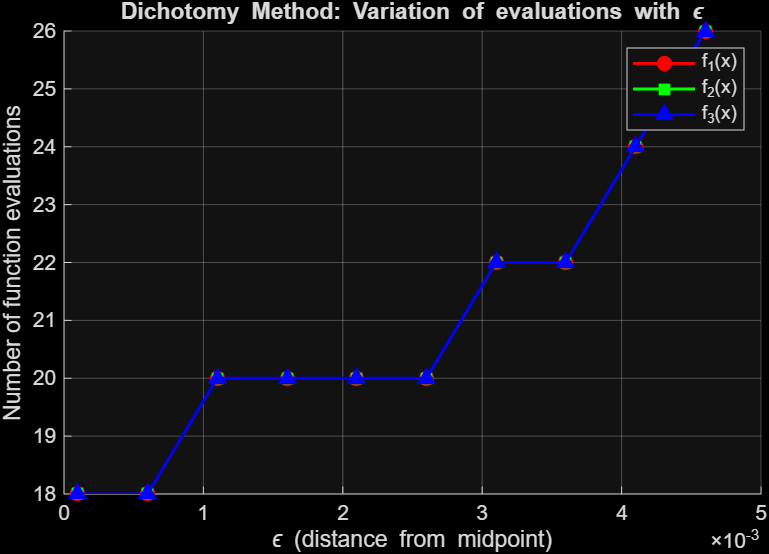
\includegraphics[width=0.7\textwidth]{assets/dichotomy/dichotomy_e.png}
    \caption{Number of function evaluations as a function of $\varepsilon$, with fixed $l = 0.01$.}
    \label{fig:dichotomy_e}
\end{figure}

Figure~\ref{fig:dichotomy_e} shows the number of function evaluations required for each test function when the tolerance is fixed at $l = 0.01$ and $\varepsilon$ varies from $0.0001$ to $0.005$. It can be observed that larger values of $\varepsilon$ result in a higher number of function evaluations. This occurs because a larger $\varepsilon$ increases the distance between the two evaluation points, which affects the interval reduction per iteration and leads to more iterations being needed to satisfy the stopping criterion.

\vspace{1em}
\begin{figure}[h!]
    \centering
    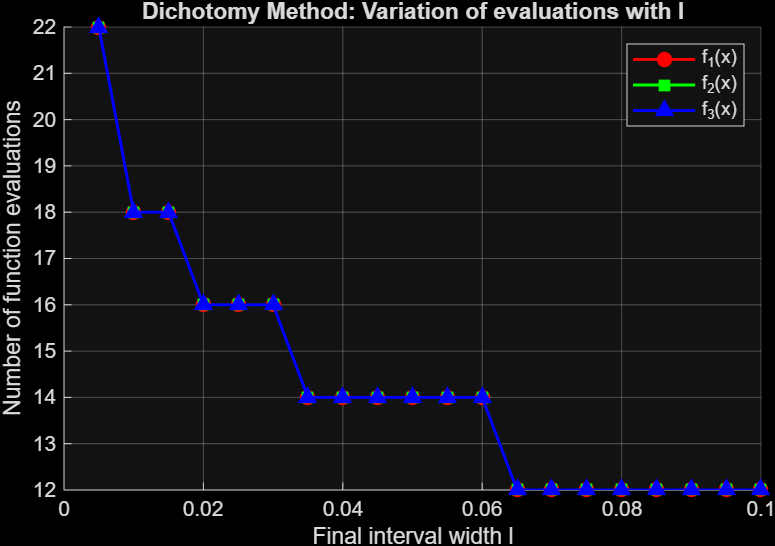
\includegraphics[width=0.7\textwidth]{assets/dichotomy/dichotomy_l.png}
    \caption{Number of function evaluations as a function of $l$, with fixed $\varepsilon = 0.001$.}
    \label{fig:dichotomy_l}
\end{figure}

\newpage

Figure~\ref{fig:dichotomy_l} illustrates how the number of function evaluations depends on the interval tolerance $l$, for a fixed $\varepsilon = 0.001$. Smaller tolerance values lead to more iterations and thus more function evaluations, which is consistent with the stopping criterion of the method.
\vspace{1em}

%--- f1 ---
\begin{figure}[h!]
    \centering
    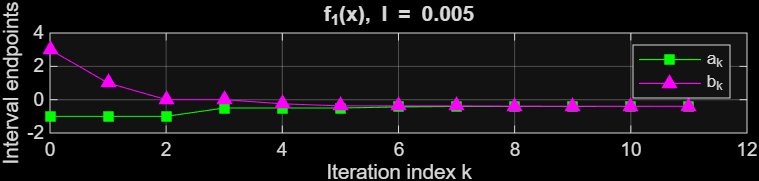
\includegraphics[width=0.7\textwidth]{assets/dichotomy/dichotomyf1.1.png}\par
    \vspace{0.5em}
    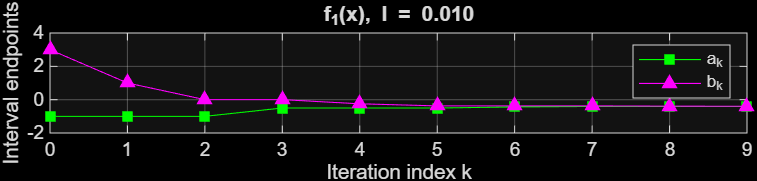
\includegraphics[width=0.7\textwidth]{assets/dichotomy/dichotomyf1.2.png}\par
    \vspace{0.5em}
    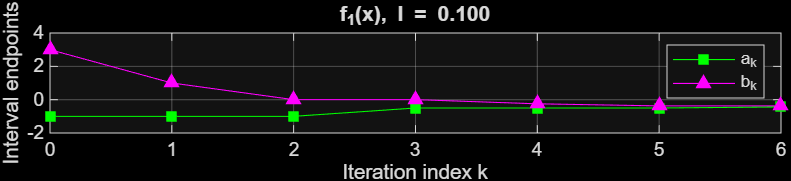
\includegraphics[width=0.7\textwidth]{assets/dichotomy/dichotomyf1.3.png}\par

    \caption{Convergence of interval endpoints $a$ and $b$ for $f_1(x)$ with Dichotomy Method, for different values of the tolerance $l$ and $\varepsilon = 0.001$.}
    \label{fig:dichotomy_intervals_f1}
\end{figure}

%--- f2 ---
\begin{figure}[h!]
    \centering
    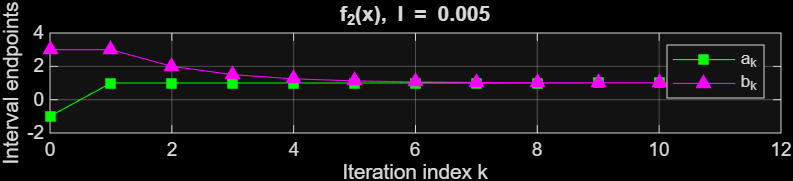
\includegraphics[width=0.7\textwidth]{assets/dichotomy/dichotomyf2.1.png}\par
    \vspace{0.5em}
    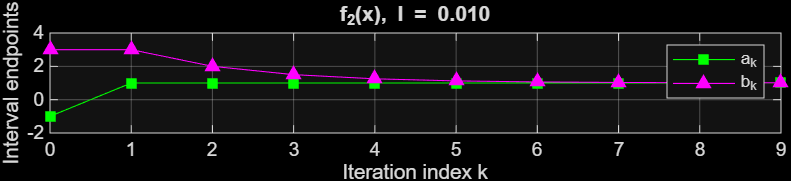
\includegraphics[width=0.7\textwidth]{assets/dichotomy/dichotomyf2.2.png}\par
    \vspace{0.5em}
    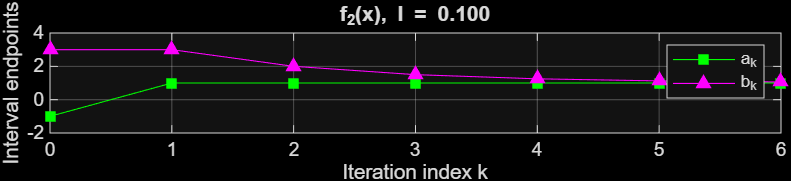
\includegraphics[width=0.7\textwidth]{assets/dichotomy/dichotomyf2.3.png}\par

    \caption{Convergence of interval endpoints $a$ and $b$ for $f_2(x)$ with Dichotomy Method, for different values of the tolerance $l$ and $\varepsilon = 0.001$.}
    \label{fig:dichotomy_intervals_f2}
\end{figure}

%--- f3 ---
\begin{figure}[h!]
    \centering
    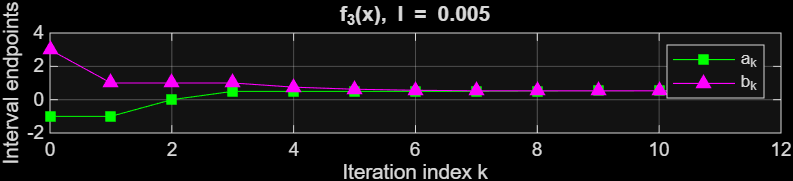
\includegraphics[width=0.7\textwidth]{assets/dichotomy/dichotomyf3.1.png}\par
    \vspace{0.5em}
    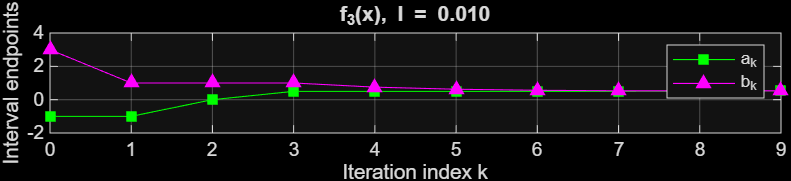
\includegraphics[width=0.7\textwidth]{assets/dichotomy/dichotomyf3.2.png}\par
    \vspace{0.5em}
    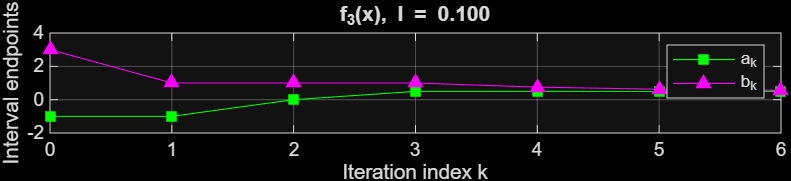
\includegraphics[width=0.7\textwidth]{assets/dichotomy/dichotomyf3.3.png}\par

    \caption{Convergence of interval endpoints $a$ and $b$ for $f_3(x)$ with Dichotomy Method, for different values of the tolerance $l$ and $\varepsilon = 0.001$.}
    \label{fig:dichotomy_intervals_f3}
\end{figure}

Figure~\ref{fig:dichotomy_intervals_f1}--\ref{fig:dichotomy_intervals_f3} show the evolution of the interval endpoints $a$ and $b$ at each iteration for all three test functions, for different values of the tolerance $l$ with $\varepsilon = 0.001$.  
It can be observed that for smaller values of $l$, the interval endpoints converge more slowly, requiring more iterations to reach the stopping criterion. Conversely, for larger values of $l$, the intervals converge faster, as the stopping condition is satisfied sooner.

\section{Golden Section Method}

\subsection{Method Description}

The Golden Section Method is an optimization technique for finding the minimum of a function within a given interval $[a, b]$.  
It reduces the search interval iteratively using the golden ratio $\phi = \frac{\sqrt{5}-1}{2} \approx 0.618$, which allows reusing function evaluations from previous iterations efficiently.

At each iteration, two points are chosen inside the current interval:
\[
x_1 = b - \phi (b-a), \quad
x_2 = a + \phi (b-a),
\]
and the function values $f(x_1)$ and $f(x_2)$ are computed. The interval is updated depending on the comparison:
\[
\text{If } f(x_1) < f(x_2), \text{ then } b = x_2, \quad \text{otherwise } a = x_1.
\]

This process continues until the interval satisfies the stopping condition:
\[
(b - a) < l,
\]
where $l$ is the desired tolerance.  
The midpoint of the final interval is taken as the estimated minimizer:
\[
x_{\text{min}} = \frac{a + b}{2}.
\]

The following code, shown in Listing \ref{lst:golden}, presents the MATLAB implementation of the Golden Section Method.

\begin{lstlisting}[language=Matlab, caption={Implementation of the Golden Section Method in MATLAB}, label={lst:golden}]
function [min_x, min_f, num_calculations, k, ak_vector, bk_vector] = golden_section(f, a, b, l)

    phi = (sqrt(5)-1)/2;   % Golden ratio (~0.618)
    k = 1;
    ak_vector = a;
    bk_vector = b;
    num_calculations = 0;

    x1 = b - phi*(b-a);
    x2 = a + phi*(b-a);
    f1 = f(x1);
    f2 = f(x2);
    num_calculations = num_calculations + 2;

    while (b - a) > l
        if f1 < f2
            b = x2;
            x2 = x1;
            f2 = f1;
            x1 = b - phi*(b-a);
            f1 = f(x1);
        else
            a = x1;
            x1 = x2;
            f1 = f2;
            x2 = a + phi*(b-a);
            f2 = f(x2);
        end

        ak_vector = [ak_vector, a];
        bk_vector = [bk_vector, b];
        num_calculations = num_calculations + 1;
        k = k + 1;
    end

    min_x = (a+b)/2;
    min_f = f(min_x);
end
\end{lstlisting}

\subsection{Plots and Observations}

The numerical results of the Golden Section Method applied to the three test functions are presented below.  
We focus on the number of function evaluations as a function of the interval tolerance $l$, along with the convergence behavior of the interval endpoints.

\newpage

\begin{figure}[h!]
    \centering
    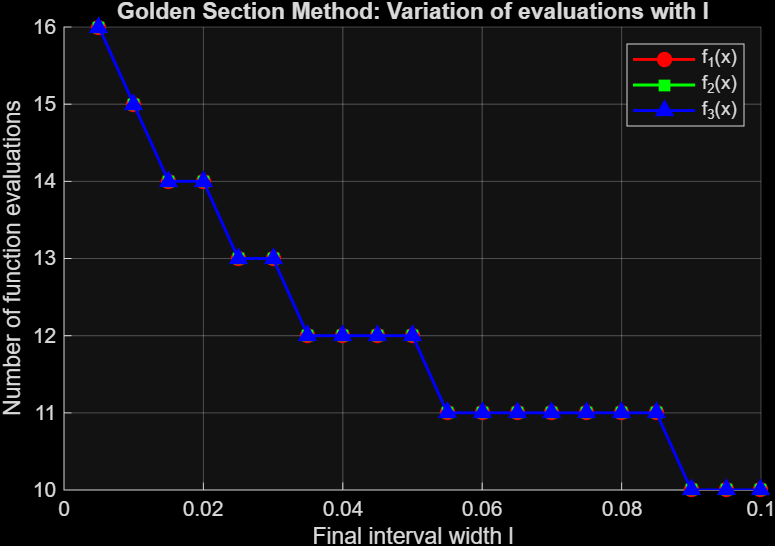
\includegraphics[width=0.7\textwidth]{assets/goldenSection/goldenSection_l.png}
    \caption{Number of function evaluations as a function of $l$, with the Golden Section Method.}
    \label{fig:golden_l}
\end{figure}

Figure~\ref{fig:golden_l} shows that smaller values of $l$ require more function evaluations, as the stopping criterion demands more iterations for tighter tolerances.

\vspace{1em}
%--- f1 ---
\begin{figure}[h!]
    \centering
    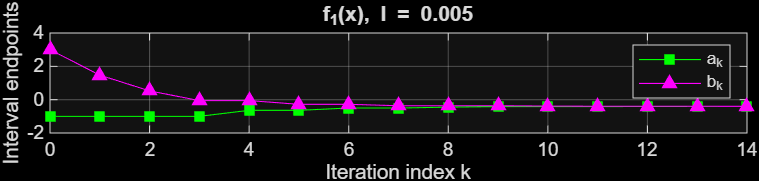
\includegraphics[width=0.7\textwidth]{assets/goldenSection/goldenSectionf1.1.png}\par
    \vspace{0.5em}
    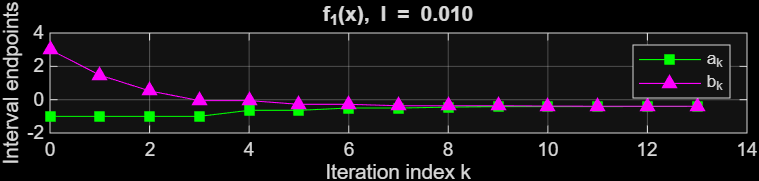
\includegraphics[width=0.7\textwidth]{assets/goldenSection/goldenSectionf1.2.png}\par
    \vspace{0.5em}
    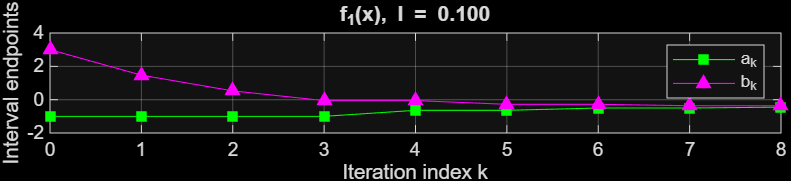
\includegraphics[width=0.7\textwidth]{assets/goldenSection/goldenSectionf1.3.png}\par

    \caption{Convergence of interval endpoints $a$ and $b$ for $f_1(x)$ with the Golden Section Method, for different values of the tolerance $l$.}
    \label{fig:golden_intervals_f1}
\end{figure}

%--- f2 ---
\begin{figure}[h!]
    \centering
    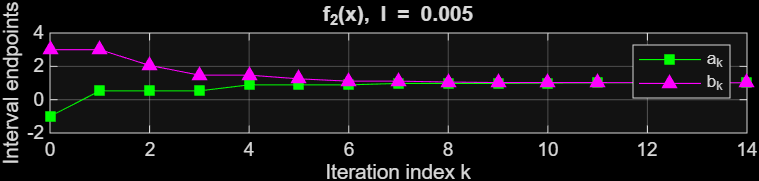
\includegraphics[width=0.7\textwidth]{assets/goldenSection/goldenSectionf2.1.png}\par
    \vspace{0.5em}
    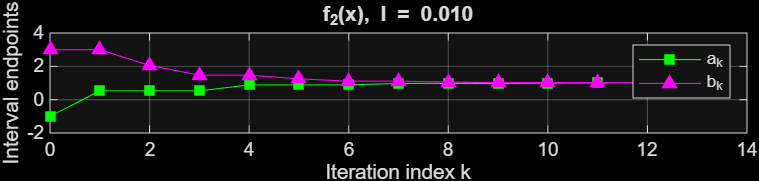
\includegraphics[width=0.7\textwidth]{assets/goldenSection/goldenSectionf2.2.png}\par
    \vspace{0.5em}
    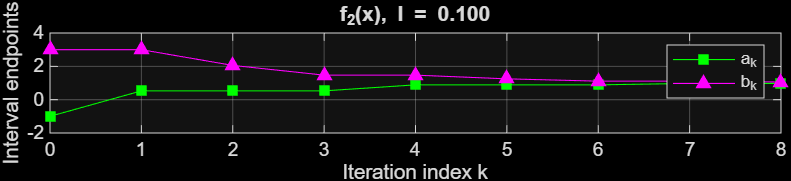
\includegraphics[width=0.7\textwidth]{assets/goldenSection/goldenSectionf2.3.png}\par

    \caption{Convergence of interval endpoints $a$ and $b$ for $f_2(x)$ with the Golden Section Method, for different values of the tolerance $l$.}
    \label{fig:golden_intervals_f2}
\end{figure}

%--- f3 ---
\begin{figure}[h!]
    \centering
    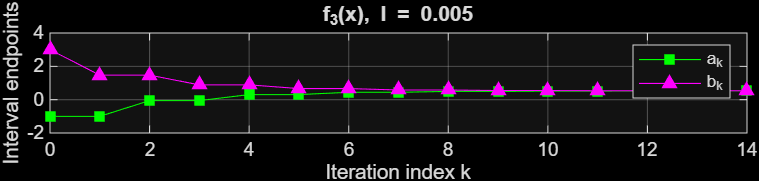
\includegraphics[width=0.7\textwidth]{assets/goldenSection/goldenSectionf3.1.png}\par
    \vspace{0.5em}
    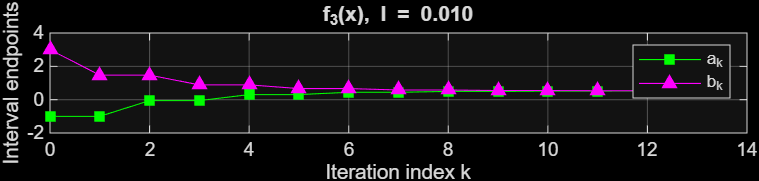
\includegraphics[width=0.7\textwidth]{assets/goldenSection/goldenSectionf3.2.png}\par
    \vspace{0.5em}
    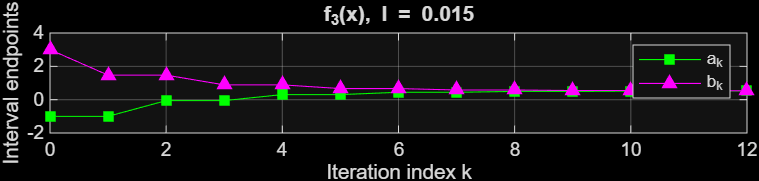
\includegraphics[width=0.7\textwidth]{assets/goldenSection/goldenSectionf3.3.png}\par

    \caption{Convergence of interval endpoints $a$ and $b$ for $f_3(x)$ with the Golden Section Method, for different values of the tolerance $l$.}
    \label{fig:golden_intervals_f3}
\end{figure}

Figure~\ref{fig:golden_intervals_f1}--\ref{fig:golden_intervals_f3} show the evolution of the interval endpoints $a$ and $b$ for all three functions.  
As with the Dichotomy Method, smaller tolerance $l$ leads to slower convergence of the interval endpoints, requiring more iterations, while larger $l$ values result in faster convergence.
\newpage

\section{Fibonacci Method}

\subsection{Method Description}

The Fibonacci Method is an iterative optimization technique used to locate the minimum of a function within a given interval $[a, b]$.  
It is similar in principle to the Golden Section Method, but it chooses evaluation points based on ratios of consecutive Fibonacci numbers to minimize the number of function evaluations.

The method generates a sequence of Fibonacci numbers $F_1, F_2, \dots, F_n$ such that
\[
F_n > \frac{b-a}{l},
\]
where $l$ is the desired interval tolerance. At each iteration, two interior points are selected as:
\[
x_1 = a + \frac{F_{n-2}}{F_n} (b-a), \quad
x_2 = a + \frac{F_{n-1}}{F_n} (b-a),
\]
and the function values $f(x_1)$ and $f(x_2)$ are compared.  
Depending on the comparison, the interval is updated by discarding the subinterval that does not contain the minimum, and new points are calculated using the ratios of the remaining Fibonacci numbers.  

The process continues until the interval length satisfies the stopping criterion:
\[
(b - a) < l.
\]
The midpoint of the final interval is taken as the estimated minimizer:
\[
x_{\text{min}} = \frac{a+b}{2}.
\]

The following code, shown in Listing \ref{lst:fibonacci}, presents the MATLAB implementation of the Fibonacci Method.

\begin{lstlisting}[language=Matlab, caption={Implementation of the Fibonacci Method in MATLAB}, label={lst:fibonacci}]
function [min_x, min_f, num_calculations, k, ak_vector, bk_vector] = fibonacci_method(f, a, b, l)

    % Generate Fibonacci numbers until F(n) > (b-a)/l
    F = [1, 1];
    while F(end) < (b-a)/l
        F = [F, F(end) + F(end-1)];
    end
    n = length(F);

    ak_vector = a;
    bk_vector = b;
    num_calculations = 0;

    % Initial interior points
    x1 = a + F(n-2)/F(n)*(b-a);
    x2 = a + F(n-1)/F(n)*(b-a);
    f1 = f(x1);
    f2 = f(x2);
    num_calculations = num_calculations + 2;

    for iter= 2:n-2
        if f1 < f2
            b = x2;
            x2 = x1;
            f2 = f1;
            x1 = a + F(n-iter-1)/F(n-iter+1)*(b-a);
            f1 = f(x1);
        else
            a = x1;
            x1 = x2;
            f1 = f2;
            x2 = a + F(n-iter)/F(n-iter+1)*(b-a);
            f2 = f(x2);
        end

        ak_vector = [ak_vector, a];
        bk_vector = [bk_vector, b];
        num_calculations = num_calculations + 1;
    end

    k = length(ak_vector);
    min_x = (a+b)/2;
    min_f = f(min_x);
end
\end{lstlisting}

\subsection{Plots and Observations}

The numerical results of the Fibonacci Method for the three test functions are presented below.  
The analysis focuses on the number of function evaluations as a function of the interval tolerance $l$, along with the convergence of the interval endpoints.

\begin{figure}[h!]
    \centering
    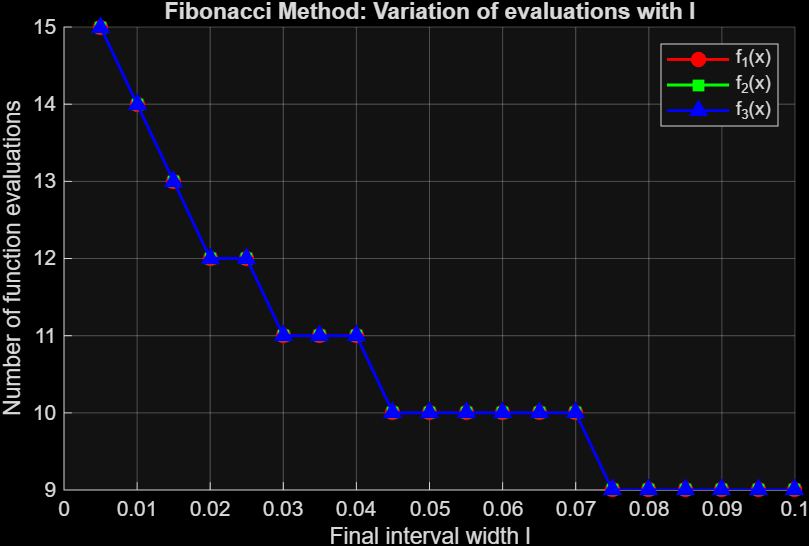
\includegraphics[width=0.7\textwidth]{assets/fibonacci/fibonacci_l.png}
    \caption{Number of function evaluations as a function of $l$, with the Fibonacci Method.}
    \label{fig:fibonacci_l}
\end{figure}

Figure~\ref{fig:fibonacci_l} shows that smaller values of $l$ require more function evaluations, as the stopping criterion demands more iterations for tighter tolerances.

\vspace{1em}
%--- f1 ---
\begin{figure}[h!]
    \centering
    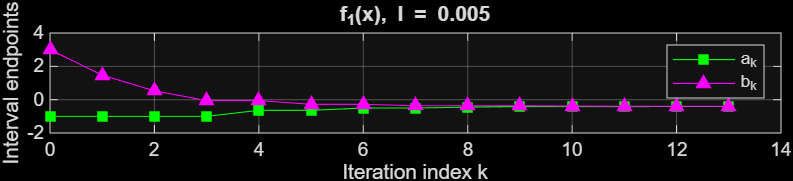
\includegraphics[width=0.7\textwidth]{assets/fibonacci/fibonaccif1.1.png}\par
    \vspace{0.5em}
    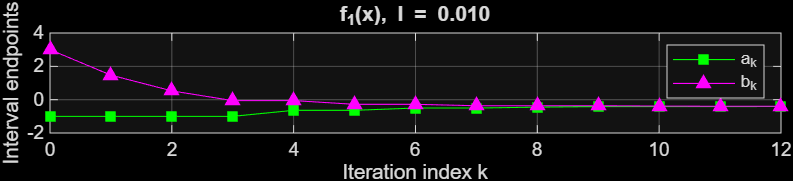
\includegraphics[width=0.7\textwidth]{assets/fibonacci/fibonaccif1.2.png}\par
    \vspace{0.5em}
    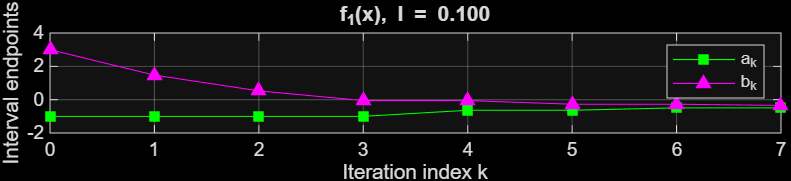
\includegraphics[width=0.7\textwidth]{assets/fibonacci/fibonaccif1.3.png}\par

    \caption{Convergence of interval endpoints $a$ and $b$ for $f_1(x)$ with the Fibonacci Method, for different values of the tolerance $l$.}
    \label{fig:fibonacci_intervals_f1}
\end{figure}

%--- f2 ---
\begin{figure}[h!]
    \centering
    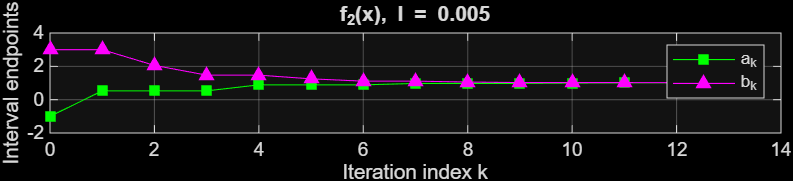
\includegraphics[width=0.7\textwidth]{assets/fibonacci/fibonaccif2.1.png}\par
    \vspace{0.5em}
    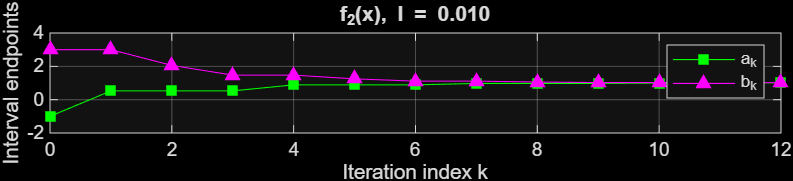
\includegraphics[width=0.7\textwidth]{assets/fibonacci/fibonaccif2.2.png}\par
    \vspace{0.5em}
    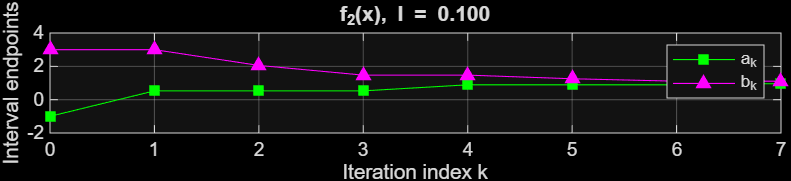
\includegraphics[width=0.7\textwidth]{assets/fibonacci/fibonaccif2.3.png}\par

    \caption{Convergence of interval endpoints $a$ and $b$ for $f_2(x)$ with the Fibonacci Method, for different values of the tolerance $l$.}
    \label{fig:fibonacci_intervals_f2}
\end{figure}

%--- f3 ---
\begin{figure}[h!]
    \centering
    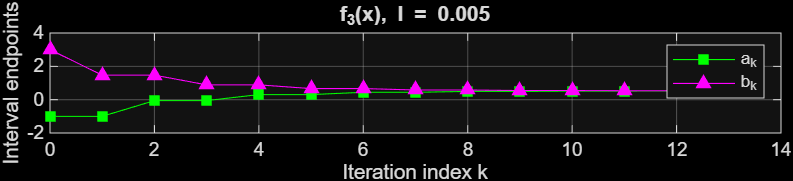
\includegraphics[width=0.7\textwidth]{assets/fibonacci/fibonaccif3.1.png}\par
    \vspace{0.5em}
    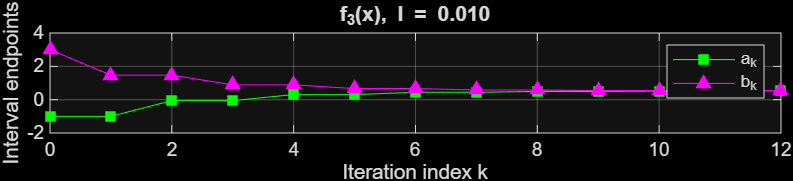
\includegraphics[width=0.7\textwidth]{assets/fibonacci/fibonaccif3.2.png}\par
    \vspace{0.5em}
    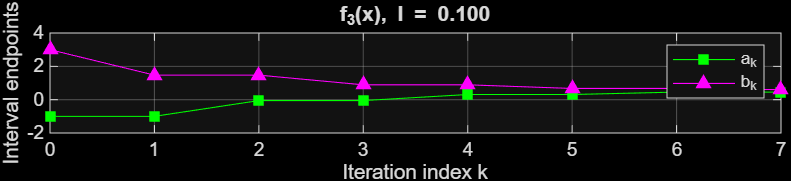
\includegraphics[width=0.7\textwidth]{assets/fibonacci/fibonaccif3.3.png}\par

    \caption{Convergence of interval endpoints $a$ and $b$ for $f_3(x)$ with the Fibonacci Method, for different values of the tolerance $l$.}
    \label{fig:fibonacci_intervals_f3}
\end{figure}

Figure~\ref{fig:fibonacci_intervals_f1}--\ref{fig:fibonacci_intervals_f3} show the evolution of the interval endpoints $a$ and $b$ for all three functions.  
As with the Dichotomy and Golden Section Methods, smaller tolerance $l$ leads to slower convergence of the interval endpoints, requiring more iterations, while larger $l$ values result in faster convergence.

\section{Dichotomy Method with Derivatives}

\subsection{Method Description}

The Dichotomy Method with Derivatives is a variant of the standard Dichotomy Method that uses the first derivative of the function to accelerate convergence.  
Instead of evaluating the function at two points around the midpoint, the method checks the sign of the derivative at the midpoint to determine the direction in which the minimum lies.

At each iteration, the midpoint of the current interval is computed:
\[
c = \frac{a+b}{2}.
\]
The derivative at the midpoint, $f'(c)$, is then evaluated. The interval is updated according to the sign of the derivative:
\[
\text{If } f'(c) < 0, \text{ then the minimum lies to the right, set } a = c, 
\]
\[
\text{If } f'(c) > 0, \text{ then the minimum lies to the left, set } b = c.
\]

The iteration continues until the interval length satisfies the tolerance:
\[
(b - a) < l.
\]
The midpoint of the final interval is taken as the estimated minimizer:
\[
x_{\text{min}} = \frac{a+b}{2}.
\]

The following code, shown in Listing \ref{lst:dich_derivative}, presents a MATLAB implementation of the Dichotomy Method with Derivatives.

\begin{lstlisting}[language=Matlab, caption={Implementation of the Dichotomy Method with Derivatives in MATLAB}, label={lst:dich_derivative}]
function [min_x, min_f, num_calculations, k, ak_vector, bk_vector] = dichotomy_derivative(f, df, a, b, l)
    ak_vector = a;
    bk_vector = b;
    num_calculations = 0;
    k = 1;

    while (b - a) > l
        c = (a+b)/2;
        dfc = df(c);
        num_calculations = num_calculations + 1;

        if dfc < 0
            a = c; % minimum in right half
        elseif dfc > 0
            b = c; % minimum in left half
        else
            a = c;
            b = c;
        end

        ak_vector = [ak_vector, a];
        bk_vector = [bk_vector, b];
        k = k + 1;
    end

    min_x = (a+b)/2;
    min_f = f(min_x);
end
\end{lstlisting}

\subsection{Plots and Observations}

The numerical results of the Dichotomy Method with Derivatives for the three test functions are presented below.  
The analysis focuses on the number of function evaluations as a function of the interval tolerance $l$, along with the convergence of the interval endpoints.

Figure~\ref{fig:dichDer_l} shows that smaller values of $l$ require more function evaluations, as the stopping criterion demands more iterations for tighter tolerances.

Figure~\ref{fig:dichDer_intervals_f1}--\ref{fig:dichDer_intervals_f3} show the evolution of the interval endpoints $a$ and $b$ for all three functions.  
As in the standard Dichotomy Method, smaller tolerance $l$ leads to slower convergence of the interval endpoints, requiring more iterations, while larger $l$ values result in faster convergence.  
Using the derivative accelerates convergence compared to the standard Dichotomy Method, as fewer function evaluations are needed to determine the interval update direction.

\begin{figure}[H]
    \centering
    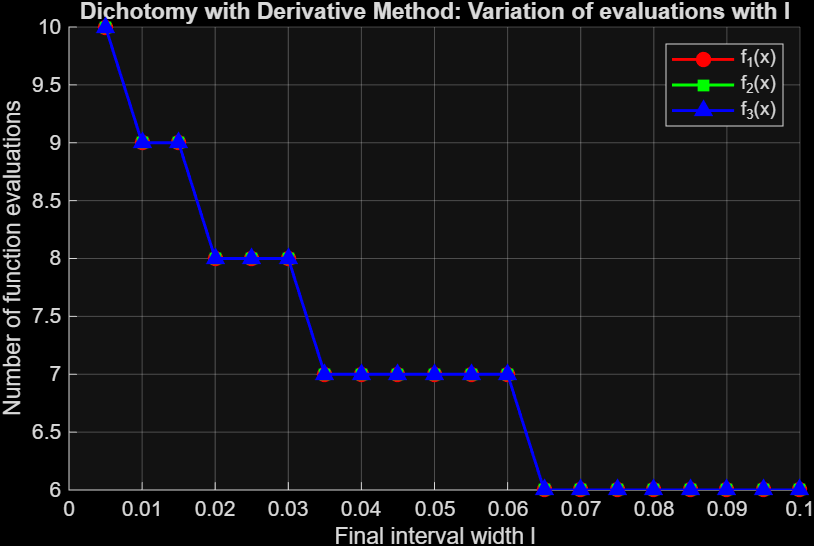
\includegraphics[width=0.7\textwidth]{assets/dichotomyDerivative/dichDer_l.png}
    \caption{Number of function evaluations as a function of $l$, using the Dichotomy Method with Derivatives.}
    \label{fig:dichDer_l}
\end{figure}

\vspace{1em}
%--- f1 ---
\begin{figure}[H]
    \centering
    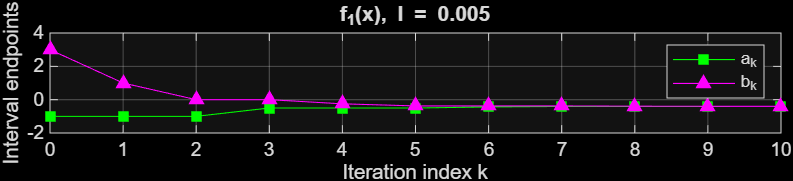
\includegraphics[width=0.7\textwidth]{assets/dichotomyDerivative/dichDerf1.1.png}\par
    \vspace{0.5em}
    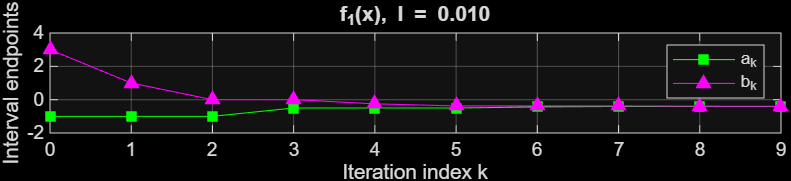
\includegraphics[width=0.7\textwidth]{assets/dichotomyDerivative/dichDerf1.2.png}\par
    \vspace{0.5em}
    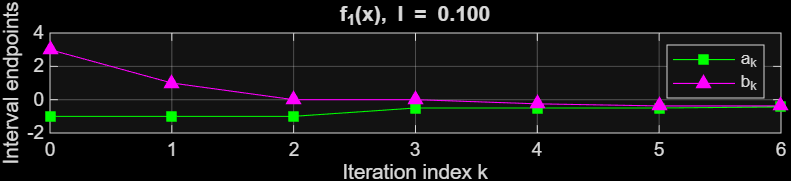
\includegraphics[width=0.7\textwidth]{assets/dichotomyDerivative/dichDerf1.3.png}\par

    \caption{Convergence of interval endpoints $a$ and $b$ for $f_1(x)$ with the Dichotomy Method using Derivatives, for different values of the tolerance $l$.}
    \label{fig:dichDer_intervals_f1}
\end{figure}

%--- f2 ---
\begin{figure}[H]
    \centering
    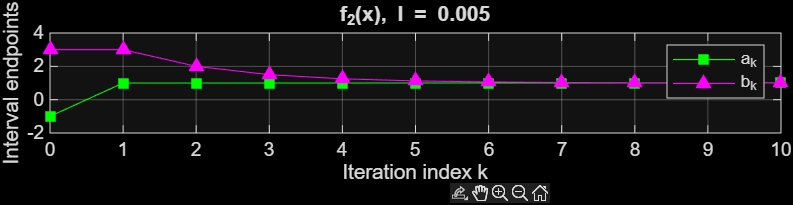
\includegraphics[width=0.7\textwidth]{assets/dichotomyDerivative/dichDerf2.1.png}\par
    \vspace{0.5em}
    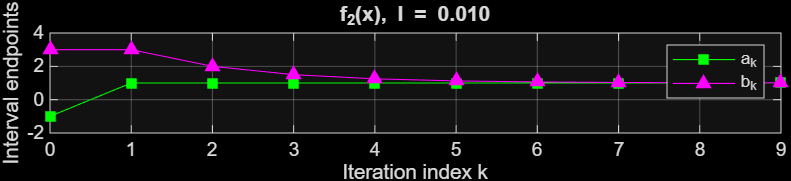
\includegraphics[width=0.7\textwidth]{assets/dichotomyDerivative/dichDerf2.2.png}\par
    \vspace{0.5em}
    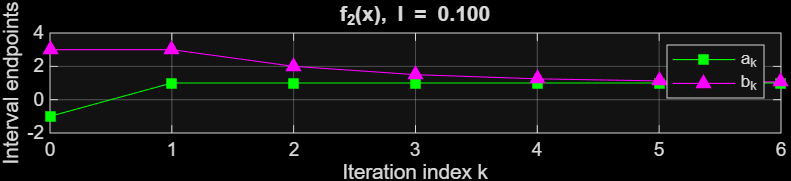
\includegraphics[width=0.7\textwidth]{assets/dichotomyDerivative/dichDerf2.3.png}\par

    \caption{Convergence of interval endpoints $a$ and $b$ for $f_2(x)$ with the Dichotomy Method using Derivatives, for different values of the tolerance $l$.}
    \label{fig:dichDer_intervals_f2}
\end{figure}

%--- f3 ---
\begin{figure}[H]
    \centering
    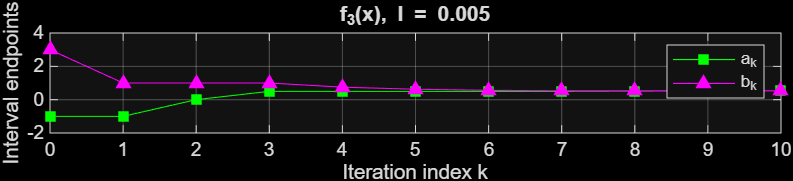
\includegraphics[width=0.7\textwidth]{assets/dichotomyDerivative/dichDerf3.1.png}\par
    \vspace{0.5em}
    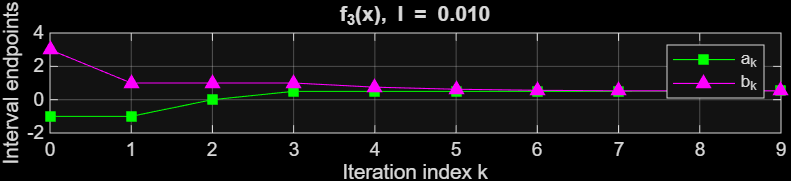
\includegraphics[width=0.7\textwidth]{assets/dichotomyDerivative/dichDerf3.2.png}\par
    \vspace{0.5em}
    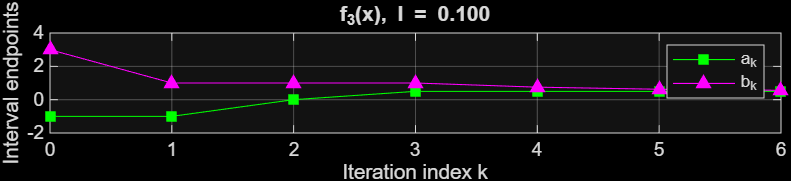
\includegraphics[width=0.7\textwidth]{assets/dichotomyDerivative/dichDerf3.3.png}\par

    \caption{Convergence of interval endpoints $a$ and $b$ for $f_3(x)$ with the Dichotomy Method using Derivatives, for different values of the tolerance $l$.}
    \label{fig:dichDer_intervals_f3}
\end{figure}

\section{Results}

Table~\ref{tab:iterations} and Table~\ref{tab:evaluations} summarize the number of iterations and the number of function evaluations, respectively, required by each optimization method to converge for three different values of the interval tolerance $l$.

\begin{table}[H]
\centering
\begin{tabular}{lccc}
\hline
\textbf{Method} & \boldmath{$l = 0.005$} & \boldmath{$l = 0.01$} & \boldmath{$l = 0.1$} \\
\hline
Dichotomy Method & 11 & 9 & 6 \\
Golden Section Method & 14 & 13 & 8 \\
Fibonacci Method & 13 & 12 & 7 \\
Dichotomy Method with Derivatives & 10 & 9 & 6 \\
\hline
\end{tabular}
\caption{Number of iterations required for convergence for each method and tolerance value $l$.}
\label{tab:iterations}
\end{table}

\begin{table}[H]
\centering
\begin{tabular}{lccc}
\hline
\textbf{Method} & \boldmath{$l = 0.005$} & \boldmath{$l = 0.01$} & \boldmath{$l = 0.1$} \\
\hline
Dichotomy Method & 22 & 18 & 12 \\
Golden Section Method & 15 & 14 & 9 \\
Fibonacci Method & 14 & 13 & 8 \\
Dichotomy Method with Derivatives & 10 & 9 & 6 \\
\hline
\end{tabular}
\caption{Number of function evaluations required for convergence for each method and tolerance value $l$.}
\label{tab:evaluations}
\end{table}

\subsection{Comparison of the Four Methods}

The results presented in Tables~\ref{tab:evaluations} allow us to compare the behavior of the four optimization methods with respect to the number of iterations and the number of function evaluations required for convergence.

First, regarding the computational cost per iteration:

\begin{itemize}
    \item \textbf{Dichotomy Method} evaluates the function twice per iteration (at the symmetrically placed points $x_1$ and $x_2$).
    
    \item \textbf{Golden Section Method} and \textbf{Fibonacci Method} evaluate the function twice only in the first iteration, and then only once per iteration, since they reuse a previously computed function value in each update step.
    
    \item \textbf{Dichotomy Method with Derivatives} evaluates the derivative only once per iteration, making each iteration cheaper compared to the standard Dichotomy Method.
\end{itemize}

These differences in per-iteration cost explain the results observed in the second table, where the total number of function evaluations differs significantly even when the number of iterations is similar.

\subsection{Convergence Speed}

A consistent trend across all values of the tolerance $l$ is observed:

\begin{itemize}
    \item \textbf{The Dichotomy Method with Derivatives converges faster} than the other three methods, both in terms of iterations and function evaluations.  
    This is expected, since using derivative information allows the method to determine the search direction more efficiently.

    \item \textbf{Golden Section} and \textbf{Fibonacci Methods} exhibit very similar convergence behavior, both in iterations and function evaluations.  
    This similarity arises because both methods use a fixed reduction ratio for updating the interval:
    \begin{itemize}
        \item the Golden Section Method uses the golden ratio factor,
        \item the Fibonacci Method uses ratios of consecutive Fibonacci numbers, which converge to the golden ratio as $n \to \infty$.
    \end{itemize}
    Therefore, both methods reduce the interval in a comparable way.
\end{itemize}

\subsection{General Conclusions}

\begin{itemize}
    \item For stricter tolerances (smaller $l$), all methods require more iterations and function evaluations, as expected.

    \item Among the \textbf{derivative-free} methods, the Golden Section and Fibonacci Methods are more efficient than the standard Dichotomy Method.

    \item The \textbf{Dichotomy Method with Derivatives} is the most efficient overall, consistently achieving convergence with the smallest number of function evaluations.
\end{itemize}


\end{document}
